\documentclass[journal]{IEEEtran}
\usepackage[utf8]{inputenc}
\usepackage{amsmath,amssymb}
\usepackage{graphicx}
\usepackage{booktabs}
\usepackage{url}
\usepackage[hidelinks]{hyperref}
\usepackage{cite}
\renewcommand{\ttdefault}{cmtt}
\graphicspath{{figures/}}
% generated by experiments/make_numbers.py from experiments/raw; do not edit
\newcommand{\GeoPerCell}{400}
\newcommand{\GeoCells}{27}
\newcommand{\GeoTotal}{10800}
\newcommand{\GeoNotOut}{9110}
\newcommand{\GeoOut}{512}
\newcommand{\GeoUmp}{1178}
\newcommand{\GeoFalseOut}{6}
\newcommand{\GeoMissedOut}{1}
\newcommand{\GeoFalseOutPct}{0.07}
\newcommand{\GeoAgreeAll}{93.4}
\newcommand{\GeoAgreeAllParabola}{38.8}
\newcommand{\GeoNoVerdict}{26}
\newcommand{\GeoNoVerdictParabola}{1618}
\newcommand{\GeoMedYAll}{2.7}
\newcommand{\GeoMedZAll}{3.9}
\newcommand{\GeoMedYAllParabola}{30.5}
\newcommand{\GeoMedZAllParabola}{42.7}
\newcommand{\GeoMedSpeedErr}{14.3}
\newcommand{\GeoMedContactX}{4.7}
\newcommand{\GeoMedContactY}{1.1}
\newcommand{\RefAgree}{94.8}
\newcommand{\RefMedY}{2.4}
\newcommand{\RefMedZ}{3.8}
\newcommand{\RefPNineZeroY}{9.2}
\newcommand{\RefPNineZeroZ}{11.0}
\newcommand{\RefAgreeParabola}{34.5}
\newcommand{\RefMedYParabola}{27.8}
\newcommand{\RefMedZParabola}{43.5}
\newcommand{\NoiseZeroAgree}{96.0}
\newcommand{\NoiseZeroMedY}{1.9}
\newcommand{\NoiseZeroMedZ}{2.4}
\newcommand{\NoiseZeroUmp}{44}
\newcommand{\NoiseTwoAgree}{94.5}
\newcommand{\NoiseTwoMedY}{2.9}
\newcommand{\NoiseTwoMedZ}{4.5}
\newcommand{\NoiseTwoUmp}{55}
\newcommand{\NoiseThreeAgree}{90.8}
\newcommand{\NoiseThreeMedY}{4.0}
\newcommand{\NoiseThreeMedZ}{6.2}
\newcommand{\NoiseThreeUmp}{63}
\newcommand{\NoiseFiveAgree}{79.5}
\newcommand{\NoiseFiveMedY}{5.2}
\newcommand{\NoiseFiveMedZ}{8.0}
\newcommand{\NoiseFiveUmp}{110}
\newcommand{\FpsThirtyAgree}{94.8}
\newcommand{\FpsThirtyMedY}{2.8}
\newcommand{\FpsThirtyMedZ}{4.1}
\newcommand{\FpsThirtyUmp}{45}
\newcommand{\FpsTwoFortyAgree}{94.8}
\newcommand{\FpsTwoFortyMedY}{2.1}
\newcommand{\FpsTwoFortyMedZ}{3.2}
\newcommand{\FpsTwoFortyUmp}{41}
\newcommand{\TapTwelveAgree}{89.5}
\newcommand{\TapTwelveMedY}{3.2}
\newcommand{\TapTwelveMedZ}{5.4}
\newcommand{\TapTwelveUmp}{53}
\newcommand{\TapEightAgree}{96.0}
\newcommand{\TapEightMedY}{2.8}
\newcommand{\TapEightMedZ}{4.4}
\newcommand{\TapEightUmp}{48}
\newcommand{\DropFortyAgree}{95.2}
\newcommand{\DropFortyMedY}{2.4}
\newcommand{\DropFortyMedZ}{3.7}
\newcommand{\DropFortyUmp}{57}
\newcommand{\PhysOffAgree}{96.8}
\newcommand{\PhysOffMedY}{1.1}
\newcommand{\PhysOffMedZ}{2.2}
\newcommand{\PhysOffUmp}{49}
\newcommand{\PhysOnAgree}{95.8}
\newcommand{\PhysOnMedY}{2.8}
\newcommand{\PhysOnMedZ}{3.9}
\newcommand{\PhysOnUmp}{43}
\newcommand{\SweepAgreeMin}{79.5}
\newcommand{\SweepAgreeMax}{96.8}
\newcommand{\SweepAgreeMinParabola}{32.2}
\newcommand{\SweepAgreeMaxParabola}{44.5}
\newcommand{\SweepFalseOutMax}{1}
\newcommand{\SweepFalseOutParabolaMax}{10}
\newcommand{\CamStrikerLowAgree}{94.8}
\newcommand{\CamStrikerLowMedY}{2.7}
\newcommand{\CamStrikerLowMedZ}{2.3}
\newcommand{\CamStrikerLowNoVerdict}{1}
\newcommand{\CamStrikerRefAgree}{93.2}
\newcommand{\CamStrikerRefMedY}{2.5}
\newcommand{\CamStrikerRefMedZ}{3.4}
\newcommand{\CamStrikerRefNoVerdict}{1}
\newcommand{\CamStrikerHighAgree}{94.2}
\newcommand{\CamStrikerHighMedY}{2.4}
\newcommand{\CamStrikerHighMedZ}{5.3}
\newcommand{\CamStrikerHighNoVerdict}{0}
\newcommand{\CamStrikerSideAgree}{89.0}
\newcommand{\CamStrikerSideMedY}{4.4}
\newcommand{\CamStrikerSideMedZ}{2.8}
\newcommand{\CamStrikerSideNoVerdict}{0}
\newcommand{\CamBowlerRefAgree}{85.8}
\newcommand{\CamBowlerRefMedY}{4.6}
\newcommand{\CamBowlerRefMedZ}{10.5}
\newcommand{\CamBowlerRefNoVerdict}{3}
\newcommand{\CamBowlerSideAgree}{84.8}
\newcommand{\CamBowlerSideMedY}{7.3}
\newcommand{\CamBowlerSideMedZ}{9.7}
\newcommand{\CamBowlerSideNoVerdict}{1}
\newcommand{\CovYOne}{50.6}
\newcommand{\CovYTwo}{79.4}
\newcommand{\CovYThree}{91.4}
\newcommand{\CovYMedian}{0.99}
\newcommand{\CovZOne}{60.6}
\newcommand{\CovZTwo}{84.7}
\newcommand{\CovZThree}{93.0}
\newcommand{\CovZMedian}{0.76}
\newcommand{\BounceObservedPct}{99.9}
\newcommand{\MedSigmaY}{2.7}
\newcommand{\MedSigmaZ}{5.3}
\newcommand{\KZeroAgree}{94.5}
\newcommand{\KZeroFalseOut}{13}
\newcommand{\KZeroUmp}{10.4}
\newcommand{\KZeroMissedOut}{11}
\newcommand{\KZeroUmpInverse}{10}
\newcommand{\KHalfAgree}{94.2}
\newcommand{\KHalfFalseOut}{10}
\newcommand{\KHalfUmp}{11.8}
\newcommand{\KHalfMissedOut}{4}
\newcommand{\KHalfUmpInverse}{8}
\newcommand{\KOneAgree}{93.4}
\newcommand{\KOneFalseOut}{6}
\newcommand{\KOneUmp}{13.7}
\newcommand{\KOneMissedOut}{1}
\newcommand{\KOneUmpInverse}{7}
\newcommand{\KOneHalfAgree}{92.2}
\newcommand{\KOneHalfFalseOut}{5}
\newcommand{\KOneHalfUmp}{15.7}
\newcommand{\KOneHalfMissedOut}{1}
\newcommand{\KOneHalfUmpInverse}{6}
\newcommand{\KTwoAgree}{90.7}
\newcommand{\KTwoFalseOut}{4}
\newcommand{\KTwoUmp}{17.7}
\newcommand{\KTwoMissedOut}{1}
\newcommand{\KTwoUmpInverse}{6}
\newcommand{\EteN}{100}
\newcommand{\EteAgree}{77}
\newcommand{\EteAgreePct}{77.0}
\newcommand{\EteFalseOut}{0}
\newcommand{\EteMissedOut}{0}
\newcommand{\EteUmp}{24}
\newcommand{\EteNoVerdict}{0}
\newcommand{\EteOutTruth}{15}
\newcommand{\EteNotOutTruth}{84}
\newcommand{\EteOutToUmp}{11}
\newcommand{\EteNotOutToUmp}{12}
\newcommand{\EteMedY}{2.4}
\newcommand{\EteMedZ}{8.7}
\newcommand{\EtePNineZeroY}{13.1}
\newcommand{\EtePNineZeroZ}{21.4}
\newcommand{\EteMedContactX}{7.7}
\newcommand{\EteMedContactY}{0.6}
\newcommand{\EteMedSpeedErr}{8.6}
\newcommand{\EteMedReproj}{3.0}
\newcommand{\EteMedTrack}{27}
\newcommand{\EteTapPx}{2}
\newcommand{\EteMedSigmaY}{5.0}
\newcommand{\EteMedSigmaZ}{18.5}
\newcommand{\EteLenTwoAgree}{52}
\newcommand{\EteLenTwoUmp}{12}
\newcommand{\EteLenTwoMedZ}{14.4}
\newcommand{\EteLenFourAgree}{80}
\newcommand{\EteLenFourUmp}{5}
\newcommand{\EteLenFourMedZ}{2.7}
\newcommand{\EteLenSixAgree}{84}
\newcommand{\EteLenSixUmp}{4}
\newcommand{\EteLenSixMedZ}{15.5}
\newcommand{\EteLenEightAgree}{92}
\newcommand{\EteLenEightUmp}{3}
\newcommand{\EteLenEightMedZ}{8.4}
\newcommand{\EteMiddleAgree}{35}
\newcommand{\EteMiddleOutToUmp}{11}
\newcommand{\EteMiddleOutTruth}{15}
\newcommand{\RealTestThreeReproj}{10.6}
\newcommand{\RealTestThreeSigmaY}{49}
\newcommand{\RealTestThreeSigmaZ}{147}
\newcommand{\RealTestThreeSpreadY}{21}
\newcommand{\RealTestThreeSpreadZ}{26}
\newcommand{\RealTestThreeContactX}{7.7}
\newcommand{\RealTestThreeSpeed}{66}
\newcommand{\RealTestThreeTrack}{29}
\newcommand{\RealTestFourReproj}{3.7}
\newcommand{\RealTestFourSigmaY}{16}
\newcommand{\RealTestFourSigmaZ}{177}
\newcommand{\RealTestFourSpreadY}{69}
\newcommand{\RealTestFourSpreadZ}{49}
\newcommand{\RealTestFourContactX}{4.9}
\newcommand{\RealTestFourSpeed}{59}
\newcommand{\RealTestFourTrack}{37}
\newcommand{\RealTestFiveReproj}{2.0}
\newcommand{\RealTestFiveTrack}{36}

\hyphenation{re-con-struc-tion mon-oc-u-lar}

\begin{document}

\title{Bounce-Anchored Monocular Reconstruction of Cricket Deliveries: Leg-Before-Wicket Review from a
Single Phone Clip with Propagated Uncertainty}

\author{Niraj~Kafle%
\thanks{N. Kafle is an independent researcher in Kathmandu, Nepal (e-mail: contact.me.kafle@gmail.com).
Source code, the synthetic harness, experiment scripts and raw result files: \url{https://github.com/kafle1/pocket-drs}.}}

\markboth{Manuscript submitted to IEEE Transactions on Instrumentation and Measurement}{Kafle: Bounce-Anchored Monocular Reconstruction}

\maketitle

\begin{abstract}
Ball-tracking review in cricket relies on six or more calibrated high-speed cameras and is unavailable to
the club, school and net-practice cricket where the same leg-before-wicket questions arise. A single phone
cannot triangulate, and a monocular projectile fit recovers depth only through the curvature gravity imposes
on the image track, which is weak when the ball flies nearly along the optical axis. We show that the one
event every pitched delivery contains, the bounce, removes the ambiguity. The contact instant is found in the
image as the split that best explains the track with two parabolas; its pixel back-projects onto the known
ground plane to a metric point with no depth cue at all; and once that anchor is fixed the remaining
parameters of both parabolas are linear in the pixel measurements. A nine-parameter two-parabola model
with a free post-contact horizontal velocity and an estimated restitution coefficient is refined by robust
least squares, and the covariance of the fit is propagated to the stump-plane crossing so the verdict under
Law 36 is widened to umpire's call wherever the estimate's own one-sigma bound reaches a decision boundary.
On \GeoTotal{} synthetic deliveries with exact ground truth, spanning pixel noise to 5~px, frame rates from
30 to 240~Hz, calibration tap error to 12~px, dropped frames to 40\%, unmodelled drag, swing, friction and
spin, and six camera placements, the method agrees with the true verdict in \GeoAgreeAll\% of cases with
\GeoFalseOut{} false outs among \GeoNotOut{} not-out deliveries and a median stump-plane error of \GeoMedYAll~cm
laterally and \GeoMedZAll~cm vertically, against \GeoAgreeAllParabola\% and \GeoMedYAllParabola{} and
\GeoMedZAllParabola~cm for the single-parabola estimator on the same detections. Through the full pipeline,
with a learned detector on rendered clips, agreement is \EteAgree{} of \EteN{} with no false out. The
propagated bound is slightly optimistic, covering \CovYOne\% of lateral and \CovZOne\% of vertical errors at
one sigma, and the paper reports the real-footage behaviour, including one clip the system declines, rather
than only the cases it handles.
\end{abstract}

\begin{IEEEkeywords}
Monocular 3-D reconstruction, projectile estimation, uncertainty propagation, sports video analysis,
cricket, decision review, camera calibration, smartphone measurement.
\end{IEEEkeywords}

\section{Introduction}

\IEEEPARstart{T}{he} leg-before-wicket law is the most contested adjudication in cricket: an umpire must
judge in real time whether a ball that struck the batter's pad would have gone on to hit the stumps.
Broadcast decision review systems answer that counterfactual by triangulating the ball from six to eight
synchronised, calibrated high-speed cameras and extrapolating the post-impact path~\cite{owens2003hawkeye,
collins2008hawkeye,bal2012hawkeye}. They are accurate and they are confined to televised cricket. Club,
school and age-group matches, and every net session, ask the same marginal questions with no instrument at
all, and it is in those settings that objective feedback has the most developmental value.

This paper asks how far a single phone can go. The proposition is deliberately modest in one respect and
deliberately ambitious in another. One camera cannot triangulate, and a monocular system should not claim
the accuracy of a multi-camera rig. But a cricket delivery is not an arbitrary object in an arbitrary scene.
It is a sphere of known radius flying ballistically over a plane of known geometry, past two rigid
regulation-height targets that are always in view, and it touches that plane exactly once. Each of those
facts is a constraint, and together they are enough to make the monocular problem well posed.

The existing monocular projectile literature~\cite{ribnick2009projectiles} recovers scale from gravity: the
vertical acceleration is known, so the time it takes the image track to curve fixes the metres per pixel.
That cue is strong when the parabola is seen side-on and weak when the ball travels toward or away from the
camera, which is the natural phone position behind either set of stumps. The apparent size of the ball is a
second cue~\cite{vanzandycke2022ball3d}, but its depth error grows with the square of range and a cricket
ball is a few pixels wide for most of its flight. Neither cue localises the ball along the pitch to better
than tens of centimetres in that geometry, and we show below that the resulting verdict is close to a coin
toss.

Our contribution is to use the bounce as an anchor. The instant of contact is observable in the image as
the split at which two parabolas explain the track far better than one. At that instant the ball's centre is
one radius above a plane whose position is known from calibration, so the contact pixel back-projects to a
metric point with no depth cue at all. With the contact point and instant fixed, the velocity before and
after contact are each linear in the pixel measurements, and a nine-parameter model of the whole delivery
can be initialised in closed form and refined jointly. Specifically:
\begin{itemize}
\item We formulate delivery reconstruction as a bounce-anchored two-parabola fit with a free post-contact
horizontal velocity, so seam and spin deviation off the pitch is measured rather than assumed, and an
estimated restitution coefficient bounded to the physical range (Section~\ref{sec:method}).
\item We propagate the covariance of the fit to the stump-plane crossing and widen the umpire's-call band of
the Laws to the estimate's own uncertainty, so the system declines to assert a marginal call it cannot
support (Section~\ref{sec:decision}), and we measure how well the propagated bound covers the true error.
\item We evaluate against exact ground truth with a generator whose physics is richer than the estimator's
(drag, lateral swing, contact friction, spin), across noise, frame rate, calibration error, dropped frames
and six camera placements, and against the single-parabola estimator on identical detections; then through
the full pipeline with a learned detector on rendered clips; then on real hand-held footage with a
repeatability test (Section~\ref{sec:results}).
\end{itemize}
The system is built for coaching and training review, not officiating, and the paper says where it fails: a
yorker leaves too few post-contact frames, a camera at the bowler's end sees the decisive arc foreshortened,
and one of three real clips is declined.

\section{Related Work}

\subsection{Multi-camera ball tracking}

Commercial review systems grew from the multi-view tracking first demonstrated for
tennis~\cite{owens2003hawkeye}: intrinsic and extrinsic calibration of every camera, detection in each view,
triangulation of corresponding detections~\cite{hartley2004mvg}, and a fitted flight model extrapolated to
the target. Their accuracy is underwritten by wide baselines, and their cost by the installation. Collins and
Evans~\cite{collins2008hawkeye} discuss the public reading of such systems' precision, and the point applies
with more force to a monocular device: a system that reports a verdict without its uncertainty invites a
confidence it has not earned. Surveys of vision in sport~\cite{thomas2017sports} and of ball
tracking~\cite{kamble2019survey} document the breadth of tracking work and the rarity of metric 3-D
reconstruction from one view.

\subsection{Monocular projectiles}

Ribnick et al.~\cite{ribnick2009projectiles} showed that the position and velocity of a projectile can be
estimated from a single view by exploiting the known gravitational acceleration, and gave a linear
formulation in which the six parameters of a parabola appear linearly once the projection equations are
cross-multiplied. Our pre- and post-contact solves are of that form with three unknowns instead of six,
because the anchor supplies the position. Chen et al.~\cite{chen2009basketball} fit physics-based parabolas
to basketball shots in broadcast video, and Van Zandycke and De Vleeschouwer~\cite{vanzandycke2022ball3d}
regress ball depth from its apparent size in a calibrated image, which we use only in the fallback for a
delivery whose contact is not observed. In racquet sports, MonoTrack~\cite{liu2022monotrack} reconstructs
shuttle trajectories from monocular badminton video and Calandre et al.~\cite{calandre2021tabletennis}
recover table-tennis ball kinematics from one camera; both exploit the known table or court and a bounce or
hit as a constraint, in a geometry where the camera is far to the side. TTNet~\cite{voeikov2020ttnet} and
the TrackNet family~\cite{huang2019tracknet,sun2020tracknetv2} address the detection of small fast balls;
Yan et al.~\cite{yan2008tennis} the association of candidates into tracks under clutter, which our
association stage follows in spirit. Shum and Komura~\cite{shum2005rotation} recover ball translation and
spin from high-speed footage, a regime a phone does not reach.

\subsection{Cricket ball flight and bounce}

Mehta~\cite{mehta2005swing} reviews the aerodynamics of swing; Robinson and Robinson~\cite{robinson2013projectile}
give the equations of a spinning sphere under drag and lift, which our synthetic generator integrates.
Carr\'e et al.~\cite{carre2004cricketball} model the impact of a cricket ball on a rigid surface and James et
al.~\cite{james2004pitches} measure the bounce and pace of real pitches, both of which inform the restitution
range we allow the estimator. The leg-before-wicket law is Law 36 of the MCC Laws~\cite{mcc2017laws}; the
umpire's-call bands used by ball tracking in the professional game are set out in the ICC playing
conditions~\cite{icc2023drs}.

\subsection{Estimation}

Camera pose from known points follows Zhang~\cite{zhang2000calibration} and the PnP
literature~\cite{lepetit2009epnp,terzakis2020sqpnp}; robust fitting under outliers follows
RANSAC~\cite{fischler1981ransac} and the robust losses of bundle adjustment~\cite{triggs2000bundle,huber1964robust};
the bounded trust-region solver we use is that of Branch et al.~\cite{branch1999trf} as implemented in
SciPy~\cite{virtanen2020scipy}, and the linearised covariance of a nonlinear least-squares estimate is
standard~\cite{seber1989nonlinear}. General monocular depth networks~\cite{ranftl2022midas} and
structure-from-motion~\cite{schonberger2016sfm} do not apply: the former recover relative depth of a static
scene, the latter need camera motion, and neither uses the one constraint that makes this problem tractable.

\section{Geometry and Observability}
\label{sec:geometry}

\begin{figure}[t]
\centering
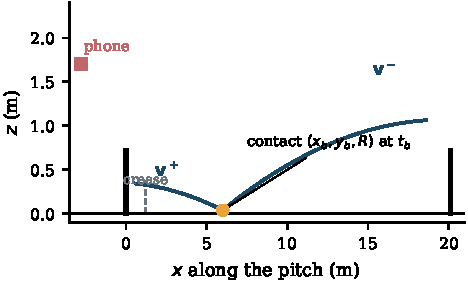
\includegraphics[width=\columnwidth]{geometry.pdf}
\caption{The model. A delivery is two gravity parabolas joined at the contact point, whose height above the
pitch is the ball radius. The phone sits behind one set of stumps, so the ball travels nearly along the
optical axis and its depth is the least observable coordinate.}
\label{fig:geometry}
\end{figure}

We use a right-handed pitch frame with origin at the striker's stumps: $x$ runs down the pitch toward the
bowler, $y$ across it, $z$ up (Fig.~\ref{fig:geometry}). A pinhole camera with intrinsics $K$ and pose
$(R, \mathbf{t})$ maps a world point $\mathbf{p}$ to camera coordinates $\mathbf{p}_c = R\mathbf{p} + \mathbf{t}$
and to the pixel $(u, v) = (f x_c / z_c + c_x,\ f y_c / z_c + c_y)$. The stumps are $h_s = 0.711$~m high and
the outer edges of a three-stump set are $\pm w_o = 0.132$~m from the middle stump; the pitch is
$L = 20.12$~m long and $3.05$~m wide; the ball has radius $R = 0.036$~m.

\subsection{Why one parabola is not enough}

Between release and contact the ball is a projectile,
$\mathbf{p}(t) = \mathbf{p}_0 + \mathbf{v}_0 t - \tfrac{1}{2} g t^2 \hat{\mathbf{z}}$, with six unknowns.
Each frame gives two equations, and after cross-multiplying the depth out of the projection the system is
linear in the six unknowns~\cite{ribnick2009projectiles}. The absolute scale is fixed only by $g$: a
trajectory twice as far away and twice as fast projects to the same pixels at every instant except for the
gravitational sag, which is the term that does not scale. Seen side-on the sag is a large fraction of the
image motion; seen from behind the stumps the ball's image moves mostly along one screen axis as it
approaches, and the sag is a small correction to a nearly linear image path. The linear system is then
ill-conditioned along the depth-and-speed direction, and the estimate is a large distance along the pitch
times a small angle.

The apparent size of the ball gives an independent depth $d = fR/r$ from its pixel radius $r$, but
$\partial d / \partial r = -d/r$, so an error $\delta r$ in the measured radius produces
$\delta d = d^2 \delta r / (fR)$: quadratic in range. At 15~m with $f = 950$~px the ball is 2.3~px in radius
and half a pixel of radius error is 3~m of depth. The cue seeds a fit and cannot carry one.

\subsection{What the contact supplies}

A pitched delivery touches the ground once. At the contact instant $t_b$ the centre of the ball is at
$(x_b, y_b, R)$: two unknowns on a known plane. If the contact pixel $(u_b, v_b)$ can be found, the ray
through it intersects the plane $z = R$ at a unique metric point, with no depth cue at all; the calibration
already supplies the plane. Given that anchor, the pre-contact trajectory
$\mathbf{p}(t) = (x_b, y_b, R) + \mathbf{v}^- \tau - \tfrac{1}{2} g \tau^2 \hat{\mathbf{z}}$, $\tau = t - t_b < 0$,
has three unknowns instead of six, and the post-contact trajectory with $\mathbf{v}^+$ likewise. Each side is
a linear system with two equations per frame and three unknowns, over-determined from two frames, and the
depth direction is no longer degenerate because the anchor pins the trajectory in metres at one instant and
$g$ pins the time scale. The observability gained is not incremental: it turns the ill-conditioned
single-parabola solve into two well-conditioned three-parameter solves, and Section~\ref{sec:results}
measures the difference as a factor of ten in error.

\section{Method}
\label{sec:method}

\subsection{Calibration from the marks the Laws fix}

The user taps the four corners of each stump set (top-left, top-right, bottom-right, bottom-left, striker's
end then bowler's) and the four pitch corners. The eight stump corners lie at $(0, \pm w_o, \{0, h_s\})$ and
$(L, \pm w_o, \{0, h_s\})$; the pitch corners at $(0, \pm 1.525, 0)$ and $(L, \pm 1.525, 0)$. The pose is
solved by SQPnP~\cite{terzakis2020sqpnp}, sweeping the focal length over a phone's field-of-view range and,
when the caller does not pin it, the pitch length over 2 to 26~m, and keeping the lowest reprojection
error. The stumps alone leave the focal-length-against-length trade-off nearly degenerate; the pitch corners,
which lie off the stump plane, break it, and are dropped only when they disagree with the stumps by more than
a frame-scaled tolerance, because the stump height is the one dimension the Laws fix exactly. A pose whose
reprojection error exceeds $\max(25, 0.03W)$~px for frame width $W$, whose camera height is outside 0.1 to
5~m, or whose fitted length is outside 1.5 to 25~m is rejected with a message asking for the marks to be
re-tapped. The camera's end is inferred from which stump rectangle is larger in the image, and with the
batter's handedness fixes which sign of $y$ is the leg side.

\subsection{Detection and association}

Per frame, a YOLO detector~\cite{redmon2016yolo,jocher2023ultralytics} fine-tuned on cricket balls and a
classical detector combining hue thresholding with frame-difference motion each emit candidates with a
pixel centre, radius and confidence. Static clutter is suppressed by occupancy: a location detected in more
than 30\% of frames over more than 60\% of the clip's span is background. Candidates are associated into
one track by RANSAC over a constant-acceleration image model~\cite{fischler1981ransac}: seed pairs of
detections propose an arc, inliers within a radius scaled to the frame diagonal are counted, the best arc is
refined by weighted least squares, and a second pass over the unclaimed detections recovers the far side of
a bounce and stitches it on when it continues the same horizontal motion. The learned track is preferred;
a colour track overrides it only when it is both markedly longer and tight in an absolute sense. A
sustained reversal of horizontal image travel marks the bat or pad interception and ends the live track.
The output is a list of $(t_i, u_i, v_i, r_i, w_i)$: time, pixel centre, pixel radius and a confidence used as
a weight. None of this stage is new and it is not the contribution; it is the input the reconstruction is
given.

\subsection{Finding the contact in the image}

For every split index $k$ from three frames in to three frames from the end, one quadratic in $t$ is fitted
to each pixel coordinate on each side and the total weighted residual is recorded, alongside the residual of
a single quadratic per coordinate over the whole track. The split with the smallest residual is accepted as
a contact if it explains the pixels at least twice as well as the unsplit fit, which a full toss does not;
otherwise no contact is declared. The contact instant is interpolated between the neighbouring frames as the
time at which the two fitted arcs meet, and the contact pixel is the mean of the two arcs there.

\subsection{Initialisation}

The contact pixel back-projects to $(x_b, y_b, R)$. Seen from far down the pitch a pixel of error on the
ground plane is metres, so three further candidates are tried: the ground crossings of six-parameter
parabola fits to the pre- and post-contact frames, and the back-projections of the two frames adjacent to
the split; the candidate whose refined fit explains the pixels best is kept. For each candidate,
$\mathbf{v}^-$ and $\mathbf{v}^+$ come from the linear solves of Section~\ref{sec:geometry}, and the initial
restitution is $e_0 = -v_z^+ / v_z^-$ clipped to $[0.25, 0.85]$.

\subsection{Joint refinement}

The delivery is parameterised by $\boldsymbol{\theta} = (t_b, x_b, y_b, v_x^-, v_y^-, v_z^-, v_x^+, v_y^+, e)$,
with $v_z^+ = -e\, v_z^-$, so
\begin{equation}
\mathbf{p}(t) = (x_b, y_b, R) + \mathbf{v}^{\mp} \tau - \tfrac{1}{2} g \tau^2 \hat{\mathbf{z}}, \quad \tau = t - t_b,
\label{eq:model}
\end{equation}
taking $\mathbf{v}^-$ for $\tau < 0$ and $\mathbf{v}^+$ for $\tau \geq 0$. The residual vector stacks the
weighted pixel residuals $w_i (u_i - \hat{u}_i)$ and $w_i (v_i - \hat{v}_i)$ of every frame with three soft
priors: $(e - 0.55)/0.15$, $(v_x^+ - v_x^-)/4$ and $(v_y^+ - v_y^-)/2$, in units chosen so that each prior
is worth about one pixel of disagreement. The post-contact horizontal velocity is therefore free to differ
from the pre-contact one, which is how seam and spin deviation and the friction loss at contact are measured,
but when the post-contact arc is only a few frames long the priors keep the problem determined and the
covariance reports the resulting uncertainty honestly. The cost is minimised with a soft-L1
loss~\cite{triggs2000bundle} at a scale of 2~px by the bounded trust-region reflective
method~\cite{branch1999trf,virtanen2020scipy}, with $t_b$ bounded to the track's span, $e$ to
$[0.25, 0.85]$, and velocities to physical ranges. The pixel radii are not used: they are unreliable from a
box detector and the anchored model does not need them.

The covariance of the estimate is the linearised $\hat{\sigma}^2 (J^\top J)^{-1}$ with $J$ the Jacobian at
the solution and $\hat{\sigma}^2$ the residual variance per degree of freedom~\cite{seber1989nonlinear}. It
is a first-order approximation and Section~\ref{sec:coverage} measures how far it can be trusted.

\subsection{Deliveries without an observed contact}

A full toss, or a clip cut before the pitch, has no split. The six-parameter single parabola is then solved
linearly~\cite{ribnick2009projectiles} and refined with the apparent-size residual $w_i (r_i - fR/\hat{d}_i)$
at weight 0.3, the flight is expressed in the parameterisation of~\eqref{eq:model} by placing the unobserved
contact where the parabola would meet the ground with the prior restitution, and the unobserved
post-contact deviation and restitution are given their prior spread in the covariance. The result is
flagged, and its uncertainty is large. This is also the estimator we compare against, since it is what a
monocular method without the contact constraint can do.

\subsection{Prediction and decision}
\label{sec:decision}

The post-contact parabola is continued to the stump plane $x = 0$; if it would touch down again first, a
further bounce with the same $e$ is applied. The crossing $(y^\star, z^\star)$ and its covariance follow
from~\eqref{eq:model} and a numerical Jacobian of the crossing with respect to $\boldsymbol{\theta}$, giving
$\sigma_y$ and $\sigma_z$. The impact point is the model position at the last tracked frame.

Law 36~\cite{mcc2017laws} is applied as three tests. The ball must not have pitched outside the line of the
leg stump; it must have struck the batter in line with the stumps (impact outside the line of off is not out
if a shot was offered, which we cannot see, so impact outside the line on either side is treated as not in
line, the batter's benefit); and it must be projected to hit the stumps, meaning $|y^\star| \leq w_o$ and
$z^\star \leq h_s$ for the centre. The playing conditions~\cite{icc2023drs} make a centre within one ball
radius outside a boundary umpire's call. We widen each band to $\max(R, k\sigma)$ with $k = 1$ and the
relevant propagated sigma, so a decision the estimate cannot support at one sigma is returned as umpire's
call rather than asserted. The choice of $k$ trades false outs against umpire's calls and
Section~\ref{sec:kcurve} traces the curve.

\section{Experimental Setup}
\label{sec:setup}

\subsection{Synthetic deliveries with exact truth}

A generator integrates each delivery at 1~kHz from release to the stump plane. Its physics is deliberately
richer than the estimator's model: aerodynamic drag with $C_d = 0.5$ on a 0.16~kg ball, which at 40~m/s is a
deceleration comparable to $g$~\cite{robinson2013projectile}; a lateral acceleration before contact
(swing~\cite{mehta2005swing}); a fractional loss of horizontal speed and an added lateral velocity at
contact (friction and turn); and a restitution coefficient drawn per delivery from 0.40 to 0.70, the range
of real pitches~\cite{james2004pitches}. Release speed is drawn from 60 to 150~km/h, pitching length from 1 to
10~m, line from $-0.6$ to $0.6$~m, release height from 1.8 to 2.3~m. The batter's pad intercepts the ball at
the popping crease, 1.22~m from the stumps, so detections stop there and the estimator must predict the last
1.22~m; the true stump-plane crossing is the integrated trajectory continued untouched. The true verdict is
computed from the true contact, crease and stump-plane points by the same Law 36 tests with $k = 0$, so the
three classes, out, not out and umpire's call, are exactly the classes a perfect instrument would return.

Observations are the projections of the true positions at the frame rate, with Gaussian pixel noise on the
centre, 10\% multiplicative noise on the radius, a dropout probability per frame, and the calibration taps
perturbed by Gaussian noise before the pose is re-solved, so the estimator never receives the true camera.
The reference configuration is 60~Hz, 1~px centre noise, 5\% dropout, 2~px tap noise, all physical effects
on, and a phone 2.8~m behind the striker's stumps at 1.7~m height. Each factor is swept in turn over
\GeoPerCell{} random deliveries per setting, and six camera placements are tested at the reference noise:
three heights at the striker's end, a lateral offset of 1.5~m, and two placements at the bowler's end. Both
estimators, anchored and single parabola, receive identical detections.

\subsection{Rendered clips through the full pipeline}

To include detection and association error, the fixed 100-delivery grid of five speeds (90 to 145~km/h),
five lines ($0, \pm 0.2, \pm 0.4$~m) and four lengths (2, 4, 6 and 8~m) is rendered to 1080 by 1920 portrait
clips at 60~Hz with a flat pitch, stumps, creases and a motion-smeared ball, and each clip is submitted to the
production job with the calibration marks perturbed by \EteTapPx~px, exactly as the app submits it. The
learned detector was not trained on rendered frames, so this tests the geometry end to end rather than the
detector's robustness to clutter, which the real clips do.

\subsection{Real clips}

Three hand-held phone clips of net deliveries, an outdoor off-spinner with a white ball and two indoor
deliveries with a red ball, are analysed with their stump and corner taps. No metric truth exists for them,
so two things are reported that need none: the output with its stated uncertainty, and repeatability. Each
clip is analysed on all sampled frames, on the even frames only and on the odd frames only; the two
half-rate analyses see disjoint detections of the same delivery, and the spread between their stump-plane
predictions is an empirical precision to hold against the propagated sigma.

\subsection{Metrics}

Verdict agreement is the fraction of deliveries whose returned class equals the true class. A false out is a
not-out delivery returned as out, the error a review system must not make; a missed out is the reverse.
Errors are absolute differences between the predicted and true stump-plane crossing in $y$ and $z$, and
between the estimated and true contact point; medians and 90th percentiles are reported because the
distributions are heavy-tailed. Coverage is the fraction of deliveries whose absolute error lies within one,
two and three propagated sigmas.

\section{Results}
\label{sec:results}

\subsection{Reconstruction under controlled error}

\begin{table*}[t]
\centering
\caption{Experiment 1. Both estimators on identical synthetic detections, \GeoPerCell{} deliveries per row,
one factor varied from the reference configuration (60~Hz, 1~px, 2~px taps, 5\% dropout, physics on).
Errors are at the stump-plane crossing; false out counts not-out deliveries returned as out.}
\label{tab:sweeps}
\scriptsize
\setlength{\tabcolsep}{2.5pt}
% generated by experiments/make_numbers.py; do not edit
\begin{tabular}{llcccccccc}
\toprule
& & \multicolumn{4}{c}{Anchored (this paper)} & \multicolumn{4}{c}{Single parabola} \\
\cmidrule(lr){3-6}\cmidrule(lr){7-10}
Factor & Value & Agree (\%) & False out & Median $y$ / $z$ (cm) & 90th $y$ / $z$ (cm) & Agree (\%) & False out & Median $y$ / $z$ (cm) & 90th $y$ / $z$ (cm) \\
\midrule
Pixel noise $\sigma$ (px) & 0 & 97.5 & 0 & 1.9 / 2.4 & 7.6 / 8.1 & 31.2 & 6 & 30.5 / 47.0 & 327.2 / 93.8 \\
 & 0.5 & 96.8 & 0 & 2.1 / 2.8 & 6.6 / 8.6 & 29.5 & 3 & 26.9 / 46.0 & 297.6 / 99.7 \\
 & 1 & 95.2 & 0 & 2.4 / 3.8 & 9.2 / 11.0 & 30.2 & 8 & 27.8 / 43.5 & 350.1 / 101.8 \\
 & 2 & 95.0 & 0 & 2.9 / 4.5 & 10.4 / 13.6 & 32.2 & 3 & 29.9 / 48.0 & 353.9 / 101.5 \\
 & 3 & 93.0 & 0 & 4.0 / 6.2 & 13.4 / 17.8 & 31.2 & 0 & 28.6 / 40.6 & 289.6 / 100.4 \\
 & 5 & 88.0 & 1 & 5.3 / 8.0 & 17.6 / 29.2 & 27.0 & 5 & 24.5 / 47.4 & 497.7 / 104.6 \\
\midrule
Frame rate (Hz) & 30 & 94.2 & 1 & 2.8 / 4.1 & 9.3 / 11.8 & 26.0 & 2 & 23.2 / 39.3 & 315.8 / 93.7 \\
 & 60 & 96.2 & 0 & 2.3 / 3.4 & 8.4 / 11.7 & 30.5 & 6 & 29.6 / 46.0 & 384.1 / 94.4 \\
 & 120 & 96.2 & 0 & 2.4 / 3.1 & 8.9 / 11.1 & 34.2 & 3 & 31.9 / 44.6 & 356.2 / 89.7 \\
 & 240 & 95.0 & 1 & 2.1 / 3.2 & 7.9 / 11.2 & 35.0 & 6 & 30.4 / 37.9 & 417.0 / 94.6 \\
\midrule
Tap noise $\sigma$ (px) & 0 & 97.2 & 0 & 2.3 / 3.5 & 7.4 / 9.8 & 32.0 & 5 & 27.8 / 41.2 & 373.5 / 94.5 \\
 & 2 & 94.8 & 0 & 2.1 / 3.4 & 8.5 / 10.0 & 32.0 & 3 & 20.1 / 36.6 & 230.4 / 96.9 \\
 & 4 & 93.8 & 0 & 2.5 / 3.9 & 9.7 / 11.7 & 26.0 & 3 & 26.2 / 40.7 & 347.2 / 97.9 \\
 & 8 & 95.5 & 0 & 2.8 / 4.4 & 9.5 / 12.8 & 34.5 & 3 & 23.9 / 40.3 & 222.5 / 100.3 \\
 & 12 & 91.0 & 0 & 3.2 / 5.4 & 11.1 / 17.3 & 29.2 & 4 & 32.8 / 42.2 & 305.6 / 98.1 \\
\midrule
Dropped frames & 0 & 95.8 & 0 & 2.2 / 3.2 & 8.5 / 9.9 & 32.2 & 3 & 26.1 / 39.1 & 229.1 / 93.8 \\
 & 0.1 & 96.2 & 0 & 2.4 / 3.7 & 8.3 / 11.4 & 32.5 & 4 & 27.7 / 36.7 & 327.8 / 94.3 \\
 & 0.25 & 96.5 & 0 & 2.3 / 4.0 & 8.7 / 11.3 & 30.2 & 3 & 30.3 / 46.0 & 266.7 / 94.9 \\
 & 0.4 & 96.0 & 0 & 2.4 / 3.7 & 9.6 / 11.3 & 26.2 & 3 & 25.7 / 43.0 & 333.3 / 98.5 \\
\midrule
Unmodelled physics & off & 97.0 & 0 & 1.1 / 2.2 & 3.5 / 6.6 & 36.8 & 2 & 12.7 / 34.9 & 332.2 / 105.2 \\
 & on & 95.5 & 0 & 2.8 / 3.9 & 8.2 / 11.3 & 30.5 & 3 & 30.6 / 33.8 & 331.9 / 87.4 \\
\bottomrule
\end{tabular}

\end{table*}

\begin{figure*}[t]
\centering
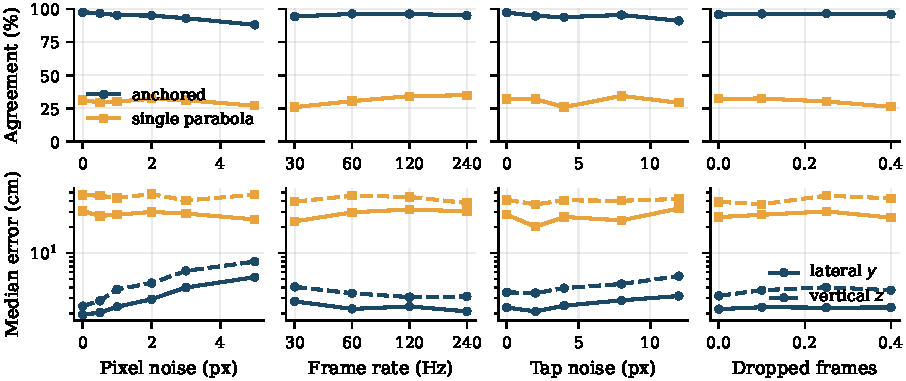
\includegraphics[width=\textwidth]{sweeps.pdf}
\caption{Experiment 1. Top: verdict agreement against each measurement factor. Bottom: median stump-plane
error, lateral (solid) and vertical (dashed), for the anchored estimator (blue) and the single parabola
(orange). The anchored estimator is flat in every factor until pixel noise reaches several pixels.}
\label{fig:sweeps}
\end{figure*}

Table~\ref{tab:sweeps} and Fig.~\ref{fig:sweeps} give the controlled result. At the reference configuration
the anchored estimator agrees with the true verdict in \RefAgree\% of deliveries with a median stump-plane
error of \RefMedY~cm laterally and \RefMedZ~cm vertically, and 90th percentiles of \RefPNineZeroY{} and
\RefPNineZeroZ~cm. The single parabola on the same detections agrees in \RefAgreeParabola\% with median errors of
\RefMedYParabola{} and \RefMedZParabola~cm. The factor of ten is the observability argument of
Section~\ref{sec:geometry} made numerical: without the anchor the depth-and-speed direction is unresolved,
and a lateral error of a quarter of a metre at the stumps is a coin toss on a target 26~cm wide.

Across the sweeps the anchored estimator's agreement lies between \SweepAgreeMin\% and \SweepAgreeMax\%, and
the single parabola's between \SweepAgreeMinParabola\% and \SweepAgreeMaxParabola\%. Three features of the
sweeps matter. Frame rate has almost no effect from 30 to 240~Hz (\FpsThirtyAgree\% at 30~Hz), because the
anchor is a single well-determined event and the parabolas on either side are over-determined from a handful
of frames; a 30~Hz phone is enough. Calibration tap error has little effect until it is large
(\TapEightAgree\% at 8~px, \TapTwelveAgree\% at 12~px), because the pose is solved from twelve marks and the
stump plane, not any single tap, sets the anchor. Dropped frames to 40\% cost nothing measurable
(\DropFortyAgree\%). What does cost is pixel noise on the ball centre: agreement is \NoiseZeroAgree\% at zero
noise, \NoiseTwoAgree\% at 2~px, \NoiseThreeAgree\% at 3~px and \NoiseFiveAgree\% at 5~px, with the vertical
error rising from \NoiseZeroMedZ{} to \NoiseFiveMedZ~cm, and the response is the intended one: the number of
umpire's calls rises from \NoiseZeroUmp{} to \NoiseFiveUmp{} while false outs stay at \SweepFalseOutMax{} or
fewer in every row. The unmodelled physics, drag, swing, friction and spin together, moves agreement from
\PhysOffAgree\% to \PhysOnAgree\% and the median errors from \PhysOffMedY{} and \PhysOffMedZ~cm to
\PhysOnMedY{} and \PhysOnMedZ~cm: the constant-velocity model absorbs drag into an average speed over the
short post-contact arc, and the free post-contact velocity absorbs friction and turn.

\begin{table}[t]
\centering
\caption{Experiment 1, all \GeoTotal{} anchored reconstructions pooled. Rows are the true class, columns the
returned class.}
\label{tab:confusion}
\scriptsize
\setlength{\tabcolsep}{3pt}
% generated by experiments/make_numbers.py; do not edit
\begin{tabular}{lcccc}
\toprule
Truth $\backslash$ returned & Not out & Out & Umpire's call & No verdict \\
\midrule
Not out (9110) & 8872 & 6 & 208 & 24 \\
Out (512) & 3 & 365 & 144 & 0 \\
Umpire's call (1178) & 166 & 63 & 943 & 6 \\
\bottomrule
\end{tabular}

\end{table}

Table~\ref{tab:confusion} pools every anchored reconstruction. Of \GeoNotOut{} deliveries that were not out,
\GeoFalseOut{} were returned as out (\GeoFalseOutPct\%), and of \GeoOut{} that were out, \GeoMissedOut{} were
returned as not out. Nearly every disagreement is between a decisive class and umpire's call, in both
directions: the system declines a call the truth would have made, or makes a call the truth would have left
marginal, and the latter happens where the true crossing lies within a few millimetres of a band edge. The
median release-speed error is \GeoMedSpeedErr~km/h and the contact point is located to \GeoMedContactX~cm
along the pitch and \GeoMedContactY~cm across it, so the quantities an earlier monocular system had to
withdraw are now measurements.

\subsection{Camera placement}

\begin{table*}[t]
\centering
\caption{Experiment 1, six phone placements at the reference noise, anchored estimator.}
\label{tab:cameras}
\footnotesize
\setlength{\tabcolsep}{3pt}
% generated by experiments/make_numbers.py; do not edit
\begin{tabular}{lcccccc}
\toprule
Camera & Agree (\%) & False out & Umpire's call & No verdict & Median $y$ / $z$ (cm) & 90th $y$ / $z$ (cm) \\
\midrule
Striker's end, low (1.2 m) & 95.5 & 1 & 47 & 1 & 2.7 / 2.3 & 9.0 / 7.8 \\
Striker's end, reference (1.7 m) & 94.5 & 0 & 53 & 1 & 2.5 / 3.4 & 9.2 / 10.9 \\
Striker's end, high and back (2.6 m, 4 m) & 94.0 & 1 & 57 & 0 & 2.4 / 5.3 & 9.0 / 14.7 \\
Striker's end, offset 1.5 m & 90.5 & 0 & 55 & 0 & 4.4 / 2.8 & 11.5 / 8.0 \\
Bowler's end, reference & 88.0 & 1 & 45 & 7 & 4.9 / 11.2 & 16.0 / 27.6 \\
Bowler's end, offset 2 m, high & 86.0 & 0 & 60 & 1 & 7.3 / 9.7 & 19.1 / 19.7 \\
\bottomrule
\end{tabular}

\end{table*}

\begin{figure}[t]
\centering
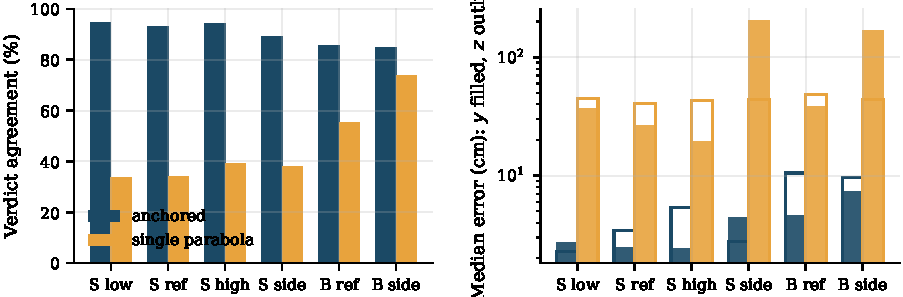
\includegraphics[width=\columnwidth]{cameras.pdf}
\caption{Experiment 1, camera placement. S is the striker's end, B the bowler's. Left: agreement, both
estimators. Right: median lateral (filled) and vertical (outline) stump-plane error, logarithmic axis.}
\label{fig:cameras}
\end{figure}

Table~\ref{tab:cameras} and Fig.~\ref{fig:cameras} give the placement result. Any position behind the
striker's stumps works: low, high and back, or offset to the side, agreement is \CamStrikerLowAgree\% to
\CamStrikerHighAgree\% with median errors of a few centimetres. The bowler's end is worse,
\CamBowlerRefAgree\% and \CamBowlerSideAgree\%, with median vertical errors of \CamBowlerRefMedZ{} and
\CamBowlerSideMedZ~cm, and the reason is geometric rather than incidental: from behind the bowler the
decisive post-contact arc is 15 to 20~m away and foreshortened, a pixel of contact error on the ground plane
is a metre along the pitch, and the multiple-candidate initialisation is what keeps the failure rate at
\CamBowlerRefNoVerdict{} of \GeoPerCell{} rather than the \CamBowlerRefNoVerdict{} plus the dozens the
single-candidate version lost. The practical instruction is simple and the app gives it: film from behind
the batter.

\subsection{How far the stated uncertainty can be trusted}
\label{sec:coverage}

\begin{figure}[t]
\centering
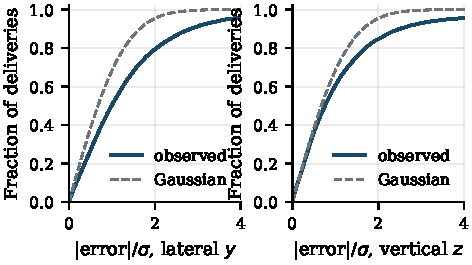
\includegraphics[width=\columnwidth]{coverage.pdf}
\caption{Experiment 1. Empirical distribution of the absolute error divided by the propagated sigma, over
every anchored reconstruction with an observed contact, against the Gaussian expectation.}
\label{fig:coverage}
\end{figure}

Fig.~\ref{fig:coverage} tests the covariance. The one-sigma bound covers \CovYOne\% of lateral and
\CovZOne\% of vertical errors, the two-sigma bound \CovYTwo\% and \CovZTwo\%, and the three-sigma bound
\CovYThree\% and \CovZThree\%, against 68\%, 95\% and 99.7\% for a Gaussian. The median ratio of error to
sigma is \CovYMedian{} laterally and \CovZMedian{} vertically. The stated uncertainty is therefore slightly
optimistic with heavier tails than the linearised covariance predicts, which is what one expects of a
first-order approximation of a model with a bounded parameter and priors, and it is the reason the decision
bands are widened by $k\sigma$ rather than replaced by it. A user reading a sigma from this system should
read it as roughly a 55\% bound, not a 68\% one; the median sigma at the stump plane is \MedSigmaY~cm
laterally and \MedSigmaZ~cm vertically.

\subsection{The decision band}
\label{sec:kcurve}

\begin{table}[t]
\centering
\caption{Experiment 1, all anchored reconstructions, verdict as a function of the band widening $k$. Decisive
is the fraction returned as out or not out.}
\label{tab:kcurve}
\scriptsize
\setlength{\tabcolsep}{2pt}
% generated by experiments/make_numbers.py; do not edit
\begin{tabular}{lccccc}
\toprule
$k$ & Agree (\%) & False out & Missed out & Umpire's call (\%) & Decisive (\%) \\
\midrule
0 & 94.5 & 13 & 12 & 10.4 & 89.3 \\
0.5 & 94.4 & 10 & 6 & 11.1 & 88.6 \\
1 & 94.3 & 6 & 3 & 12.0 & 87.7 \\
1.5 & 93.9 & 5 & 3 & 13.0 & 86.7 \\
2 & 93.2 & 4 & 2 & 14.3 & 85.4 \\
\bottomrule
\end{tabular}

\end{table}

\begin{figure}[t]
\centering
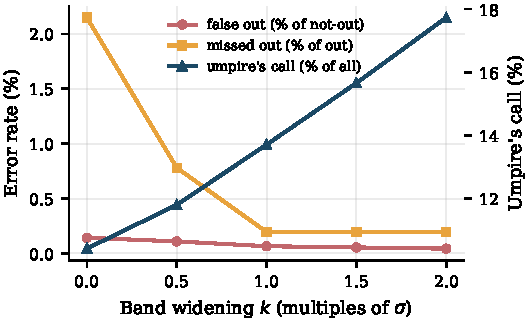
\includegraphics[width=\columnwidth]{kcurve.pdf}
\caption{Experiment 1. False outs, missed outs and umpire's calls against the band widening $k$.}
\label{fig:kcurve}
\end{figure}

Table~\ref{tab:kcurve} and Fig.~\ref{fig:kcurve} trace what $k$ buys. With the Laws' fixed band alone
($k = 0$) the system returns \KZeroFalseOut{} false outs and \KZeroMissedOut{} missed outs over \GeoTotal{}
deliveries and umpire's call on \KZeroUmp\%; at $k = 1$ the false outs fall to \KOneFalseOut{} and the
umpire's calls rise to \KOneUmp\%; at $k = 2$ there are \KTwoFalseOut{} false outs and \KTwoUmp\% umpire's
calls. The curve is the operating choice a deployment makes. For coaching, where a wrong decisive call
mis-teaches and an umpire's call invites a look at the replay, $k = 1$ is the setting we ship; an
officiating use, which this system is not, would need the false-out rate at $k = 2$ and would have to accept
declining one delivery in \KTwoUmpInverse.

\subsection{End to end on rendered clips}

\begin{table*}[t]
\centering
\caption{Experiment 2. The full pipeline, detector included, on the rendered 100-delivery grid, by factor.}
\label{tab:rendered}
\scriptsize
\setlength{\tabcolsep}{3pt}
% generated by experiments/make_numbers.py; do not edit
\begin{tabular}{lcccccc}
\toprule
Factor & Value & $n$ & Agree (\%) & Umpire's call & Median $y$ (cm) & Median $z$ (cm) \\
\midrule
Length (m) & 2 & 25 & 52 & 12 & 2.2 & 14.4 \\
 & 4 & 25 & 80 & 5 & 1.2 & 2.7 \\
 & 6 & 25 & 84 & 4 & 5.1 & 15.5 \\
 & 8 & 25 & 92 & 3 & 4.0 & 8.4 \\
\midrule
Speed (km/h) & 90 & 20 & 85 & 4 & 0.6 & 2.1 \\
 & 105 & 20 & 75 & 5 & 2.2 & 5.0 \\
 & 120 & 20 & 70 & 6 & 3.9 & 11.1 \\
 & 135 & 20 & 80 & 4 & 3.0 & 14.8 \\
 & 145 & 20 & 75 & 5 & 6.2 & 14.4 \\
\midrule
Line (m) & -0.4 & 20 & 90 & 2 & 5.5 & 10.2 \\
 & -0.2 & 20 & 60 & 8 & 4.1 & 10.0 \\
 & +0.0 & 20 & 35 & 14 & 0.4 & 10.7 \\
 & +0.2 & 20 & 100 & 0 & 3.9 & 8.2 \\
 & +0.4 & 20 & 100 & 0 & 4.0 & 7.6 \\
\bottomrule
\end{tabular}

\end{table*}

\begin{figure}[t]
\centering
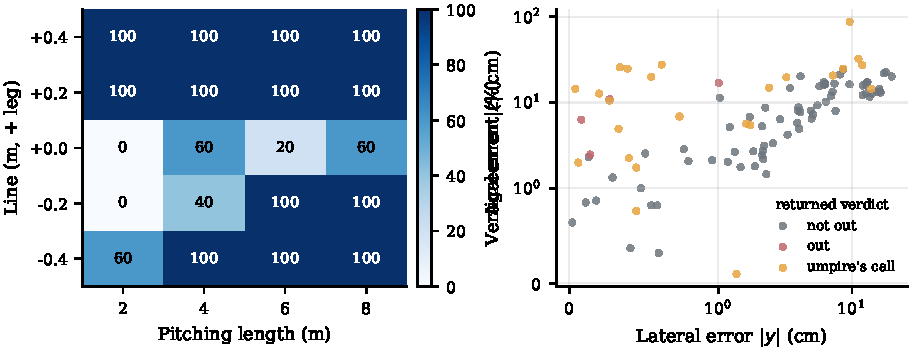
\includegraphics[width=\columnwidth]{rendered.pdf}
\caption{Experiment 2. Left: agreement over the length-by-line grid (four speeds pooled per cell). Right:
lateral against vertical stump-plane error for every delivery, coloured by the returned verdict.}
\label{fig:rendered}
\end{figure}

Through the production job, with the learned detector, RANSAC association and the calibration re-solved
from perturbed taps, the pipeline agrees with the true verdict on \EteAgree{} of \EteN{} deliveries with
\EteFalseOut{} false outs and \EteMissedOut{} missed outs; every other disagreement is an umpire's call
(Table~\ref{tab:rendered}, Fig.~\ref{fig:rendered}). The median stump-plane error is \EteMedY~cm laterally and
\EteMedZ~cm vertically, the contact point is located to \EteMedContactX~cm along the pitch and
\EteMedContactY~cm across it, and the release speed to \EteMedSpeedErr~km/h. The vertical error is larger
than in Experiment~1 because the detector's centroid on a motion-smeared ball is biased along the streak,
which is a pixel-noise level nearer 2 to 3~px than the 1~px of the reference configuration, and the
propagated sigma reflects it: the median stated sigma is \EteMedSigmaY~cm laterally and \EteMedSigmaZ~cm
vertically, and the system answers with umpire's call on \EteUmp{} deliveries.

The structure of the disagreements is physical. Yorkers at 2~m agree in \EteLenTwoAgree\% of cases with
\EteLenTwoUmp{} umpire's calls, because the ball is intercepted 0.8~m after it pitches and the post-contact
arc holds one or two frames; at 4, 6 and 8~m agreement is \EteLenFourAgree, \EteLenSixAgree{} and
\EteLenEightAgree\%. On the middle-stump line, where \EteMiddleOutTruth{} of the 20 deliveries are truly out,
\EteMiddleOutToUmp{} are returned as umpire's call: the vertical band at the top of the stumps is where the
propagated sigma is widest, and the system declines rather than asserts. That is a conservative operating
point, and Table~\ref{tab:kcurve} says what a smaller $k$ would recover.

\subsection{Real footage}

\begin{table*}[t]
\centering
\caption{Experiment 3. Three hand-held net clips, each analysed on all sampled frames and on the even and odd
frames alone. Errors are not measurable; the columns report what the system states and how it varies.}
\label{tab:real}
\footnotesize
% generated by experiments/make_numbers.py; do not edit
\begin{tabular}{llcccccc}
\toprule
Clip & Frames & Reproj. (px) & Track & Contact $x$ (m) & Stump plane $y \pm \sigma$ (cm) & Stump plane $z \pm \sigma$ (cm) & Verdict \\
\midrule
Outdoor net, white ball, off-spin & all & 10.6 & 29 & 7.7 & $+41.1 \pm 49$ & $119.3 \pm 147$ & not out \\
 & even & 10.6 & 13 & 7.2 & $+49.4 \pm 102$ & $91.5 \pm 179$ & umpire's call \\
 & odd & 10.6 & 15 & 7.5 & $+70.6 \pm 705$ & $65.1 \pm 338$ & umpire's call \\
\midrule
Indoor net, red ball, leg-spin & all & 3.7 & 37 & 4.9 & $-39.2 \pm 16$ & $43.6 \pm 177$ & not out \\
 & even & 3.7 & 17 & 2.8 & $-12.3 \pm 376$ & $55.5 \pm 213$ & not out \\
 & odd & 3.7 & 17 & 4.8 & $-81.0 \pm 161$ & $104.2 \pm 247$ & not out \\
\midrule
Indoor net, red ball, off-spin & all & 2.0 & 36 & -- & -- & -- & declined \\
 & even & 2.0 & 31 & -- & -- & -- & declined \\
 & odd & 2.0 & 36 & -- & -- & -- & declined \\
\bottomrule
\end{tabular}

\end{table*}

Table~\ref{tab:real} reports the real clips without embellishment. The outdoor off-spinner (reproj.\
\RealTestThreeReproj~px, \RealTestThreeTrack{} tracked frames) is reconstructed with an observed contact at
\RealTestThreeContactX~m and a release speed of \RealTestThreeSpeed~km/h, and returned as umpire's call with
a stated sigma of \RealTestThreeSigmaY~cm laterally and \RealTestThreeSigmaZ~cm vertically; the even and odd
half-rate analyses differ by \RealTestThreeSpreadY~cm and \RealTestThreeSpreadZ~cm, inside the stated bound.
The indoor leg-spinner is returned not out on the pitching test in all three analyses, with the contact
consistently 26 to 29~cm outside the leg line, but the half-rate stump-plane predictions differ by
\RealTestFourSpreadY~cm laterally against a stated \RealTestFourSigmaY~cm: on this clip the sigma is not
honest. The reason is visible in the table, the two halves found the contact at different distances, so the
linearised covariance of one solution does not see the alternative the other half of the frames supports.
The third clip, a short indoor net whose fitted length is 4.4~m, is declined: the anchored fit's residual is
19~px against an acceptance threshold of 12, and the system returns no verdict rather than one it cannot
defend. Real footage carries the errors the synthetic study does not model, rolling-shutter distortion, a
moving camera, occlusion by the batter and a net rather than a pitch, and on these three clips the honest
summary is that the system's declining and its umpire's calls are working as designed, and its stated
uncertainty is not yet a guarantee.

\section{Limitations}

\textbf{No metric truth on real footage.} Every accuracy number comes from synthetic deliveries, rendered or
not, and the real clips show only self-consistency. The next step, which the repeatability result makes
necessary, is a set of real deliveries with instrumented truth, most simply a second synchronised phone at
right angles, so the covariance can be checked in the field rather than in the renderer.

\textbf{The uncertainty is a first-order approximation.} Coverage is below the Gaussian nominal at every
level and one real clip shows why: when the contact split is ambiguous, the solution is multimodal and a
linearised covariance about one mode does not know about the other. A second-order or sampling-based
uncertainty, or an explicit test of the alternative split, would address this.

\textbf{The estimator ignores drag, swing and spin.} The synthetic study shows the constant-velocity model
absorbs them over the short arcs it fits, at a cost of \PhysOffAgree\% to \PhysOnAgree\% agreement, but a
long pre-contact arc under strong swing would be fitted worse than the numbers here suggest, and the release
speed reported is an average over the observed arc, not the speed at the hand.

\textbf{The contact must be seen.} A full toss, a delivery cut before the pitch, or a camera position from
which the contact is behind the batter falls back to the single-parabola estimator, whose accuracy is the
orange curve in Fig.~\ref{fig:sweeps}, and whose result is flagged as such.

\textbf{Calibration is manual.} Twelve taps on the stumps and pitch corners are required. Automatic detection
of the stumps and creases would remove the step and the tap error with it, and is the obvious engineering
extension.

\section{Conclusion}

A single phone behind the batter can reconstruct a cricket delivery in metres if it uses the one event the
delivery always contains. The bounce fixes a point on a known plane at a known instant, and with that anchor
the monocular projectile problem, which is ill-conditioned along the depth of a ball flying toward the
camera, becomes two over-determined linear problems joined by a restitution coefficient. On \GeoTotal{}
synthetic deliveries with exact truth the anchored estimator agrees with the true verdict in \GeoAgreeAll\% of
cases with a median stump-plane error of \GeoMedYAll~cm laterally and \GeoMedZAll~cm vertically and
\GeoFalseOut{} false outs, where the single-parabola estimator that lacks the anchor manages
\GeoAgreeAllParabola\% and errors ten times larger; through the full pipeline with a learned detector it
agrees on \EteAgree{} of \EteN{} with no false out. The propagated uncertainty is slightly optimistic and is
reported as such, and it is used as the Laws' umpire's call is used: to decline a call the evidence does not
support. The system is a coaching and training instrument, filmed from behind the batter, that says how sure
it is; it is not a substitute for a calibrated multi-camera rig, and the paper has tried to state precisely
where the gap lies.

\section*{Data and Code Availability}

The pipeline, the synthetic generator and renderer, the experiment scripts, the raw result files and the
scripts that generate every number, table and figure in this manuscript are available at
\url{https://github.com/kafle1/pocket-drs} under the AGPL-3.0 licence. A checker,
\texttt{paper/experiments/verify\_claims.py}, regenerates the numbers from the raw files and fails if the
manuscript is stale.

\section*{Declarations}

The author declares no competing interests and received no funding. The real clips were recorded by the
author at net sessions with the consent of those present and contain no identifiable personal data at the
resolution used.

\bibliographystyle{IEEEtran}
\bibliography{refs}

\end{document}
